\chapter{Query translation}
Following the abstraction and conversion processes established for entities and mapping, query translation can be approached in a similar manner. By comparing query concepts across \acrshort{orm} frameworks, a unified abstraction can be derived. Once this abstraction is defined, the full translation process can be formulated, along with algorithms demonstrating its application. 


\section{Query abstraction}
The analyzed frameworks offer only two main query languages - \acrshort{sql} and \acrshort{linq}. RepoDB's lambda expressions can be considered a very limited subset of \acrshort{linq}, while \acrshort{hql}, used only by NHibernate, is syntactically similar to \acrshort{sql} sees minimal adoption and is not recommended\footnote{\url{https://www.red-gate.com/simple-talk/development/dotnet-development/some-nhibernate-best-practices/\#forget-about-hql}}. As discussed in \autoref{sec:core_translation}, \acrshort{linq} is typically translated into \acrshort{sql} before the database query is executed. Therefore, \acrshort{sql} can serve as a good foundation for abstraction. However, it is not used directly, as doing so would restrict potential future extensions. A simpler, yet less general approach---executing a \acrshort{linq} query, capturing the generated \acrshort{sql}, and reusing it with a raw \acrshort{sql} query method in another \acrshort{orm}-- is an approach not considered in this work.

While entity and mapping definitions follow a relatively limited set of formats and possibilities, parsing LINQ queries becomes a challenge of parsing arbitrary C\# code. Queries must be interpreted in the context of the framework and the surrounding method in which they appear. They are rarely standalone, often referencing method arguments or external variables. Each framework uses a distinct object to represent a database connection or session. This object is responsible for query initialization and typically exposes methods for executing raw \acrshort{sql}. For \acrshort{linq} queries, it provides access to the implementation of the \texttt{IQueryable}\footnote{\url{https://learn.microsoft.com/en-us/dotnet/csharp/linq/get-started/introduction-to-linq-queries\#the-data-source}} interface, parametrized with the source entity type and extended through chained \acrshort{linq} method calls.

\autoref{tab:query_comp}, based on the framework analysis in \autoref{chapter:ormcomparison}, summarizes the structure of supported queries. Rows represent key query components, and columns correspond to specific \acrshort{orm}s. As previously mentioned, only \acrshort{sql} and \acrshort{linq} queries are considered.

Queries primarily consist of the application code that defines the \textbf{query source}, \textbf{method}, and a \textbf{generic parameter} referencing entity. The query itself can be decomposed into parts: \textbf{projection}, \textbf{selection}, \textbf{joining}, \textbf{grouping}, \textbf{ordering} and \textbf{set operations}. 

Among the frameworks that support \acrshort{linq}, it is evident that they share common semantic operations, with occasional differences in method names (e.g., \texttt{LoadWith}, \texttt{Fetch}, \texttt{Include}). Translating a \acrshort{linq} query to another \acrshort{orm}'s \acrshort{linq} implementation could, in principle, be achieved by simple method renaming, without the need for an intermediate representation. However, this approach is not further explored in this work.

%\clearpage
\begin{landscape}
\begin{table}
\centering
\caption{Comparison of key query components across different frameworks.}
\label{tab:query_comp}
\scriptsize
\def\arraystretch{1.35}
\begin{tabular}{
>{\raggedright\arraybackslash}p{20.00mm}
>{\arraybackslash}p{30.00mm}
>{\arraybackslash}p{30.00mm}
>{\arraybackslash}p{30.00mm}
>{\arraybackslash}p{30.00mm}
>{\arraybackslash}p{30.00mm}
>{\arraybackslash}p{30.00mm}
}
\toprule
  &  \textbf{Dapper}\newline raw SQL &  \textbf{PetaPoco} \newline raw SQL/Sql.Builder &   \textbf{RepoDB} \newline lambda expressions &   \textbf{LINQ to DB} \newline LINQ & \textbf{NHibernate} \newline LINQ  &   \textbf{EF Core} \newline LINQ \\
\midrule

Query source  & SqlConnection & IDatabase & SqlConnection & DataConnection &  ISession & DbContext \\
\midrule

Raw SQL method  & \texttt{SqlConnection\newline.Query()} & \texttt{IDatabase\newline.Query()} & \texttt{SqlConnection\newline.ExecuteQuery()} & \texttt{DataConnection\newline.Query()} &  \texttt{ISession\newline.CreateSQLQuery()} & \texttt{DbContext\newline.SqlQueryRaw()} \\
\midrule

LINQ method & - & - & - & \texttt{DataConnection\newline.GetTable<>()} & \texttt{ISession\newline.Query<>()} & \texttt{DbContext\newline.DBSet<>()} \\
\midrule

Source table  & FROM & FROM or entity mapping & entity mapping  & entity mapping &  entity mapping & entity mapping \\
\midrule

Projection & SELECT $\ldots$ & \texttt{Sql.Builder} automatically from entity & \texttt{Field.From()}  & default entity, modified with \texttt{Select()} & default entity, modified with \texttt{Select()} & default entity, modified with \texttt{Select()} \\
\midrule

Selection & WHERE $\ldots$ & \texttt{Sql.Builder\newline.Where()} & lambda function as query parameter \newline (\texttt{s => s.SupplierID == 10})  & \texttt{Where()} & \texttt{Where()} & \texttt{Where()} \\
\midrule

Joining & JOIN $\ldots$ ON $\ldots$ & \texttt{Sql.Builder\newline.LeftJoin().On()} & raw SQL or \mbox{QueryMultiple} & navigation property and mapping \newline + \texttt{LoadWith()} & navigation property and mapping \newline + \texttt{Fetch()} & navigation property and mapping \newline + \texttt{Include()} \\
\midrule

Grouping  & GROUP BY $\ldots$ \newline HAVING $\ldots$ & \texttt{Sql.Builder\newline.GroupBy()} & - & {GroupBy()} followed by \texttt{Where()} &  {GroupBy()} followed by \texttt{Where()} & {GroupBy()} followed by \texttt{Where()} \\
\midrule

Set operations  & UNION, INTERSECT& UNION, INTERSECT& UNION, INTERSECT & \texttt{Union()}, \texttt{Intersect()} &  \texttt{Union()}, \texttt{Intersect()} & \texttt{Union()}, \texttt{Intersect()} \\
\midrule

Ordering  & ORDER BY $\ldots$  & \texttt{Sql.Builder\newline.OrderBy()} & \texttt{OrderField\newline.Ascending()} & \texttt{OrderBy()} &  \texttt{OrderBy()} & \texttt{OrderBy()} \\

\bottomrule
\end{tabular}
\end{table}
\end{landscape}


\section{Abstract instructions}
Unlike for entities and mapping, where the intermediate representation was designed as a class-based model, queries are instead represented as a set of instructions.

The instruction must be stored in a list. On each subquery start and end, a \textit{push} and \textit{pop} methods must be called respectively to wrap a corresponding set of instructions into a \texttt{SUBQUERY} instruction. The only top-level instructions can be \texttt{SUBQUERY} and \texttt{SET\_OPERATION} instruction. \texttt{SET\_OPERATION} serves for connecting multiple queries using set operations (e.g., union, intersection).

A single subquery is composed of several different instructions, each serving a distinct purpose. The \texttt{FROM} instruction specifies the source table and an optional alias. Aliases from the original query are preserved to maintain readability and prevent ambiguity during the translation process. The \texttt{PROJECT} instruction determines which attributes are projected into the result set, optionally assigning aliases that must remain consistent throughout the query. Additionally, if a \texttt{GROUP\_BY} instruction is present, it records any aggregation functions applied to these attributes. The \texttt{PROJECT} instruction may be repeated to represent multiple projections. 

The \texttt{SELECT} instruction applies filtering conditions to rows. Due to their complexity\footnote{\url{https://learn.microsoft.com/en-us/sql/t-sql/queries/search-condition-transact-sql}}, these conditions cannot be represented by simple arguments and instead require a structured representation such as a tree of logical and comparison operators with nested operands. This representation can be a properly parenthesized expression or an object-based model, with operands potentially including constants, attributes, or references to other \texttt{SUBQUERY} instructions.

The \texttt{GROUP\_BY} references the attribute used for grouping results. It can be followed by the \texttt{HAVING} instruction, which further filters groups based on a condition tree. 
Multiple tables can be joined with the \texttt{JOIN} instruction referencing two tables, the type of join (e.g., left, inner, outer), and a condition tree specifying the join criteria. 
The \texttt{ORDER\_BY} instruction indicates an attribute by which to sort the results and the sorting direction (ascending or descending).

The complete set of proposed instructions with their respective arguments is as follows:
\begin{itemize}
    \item \textbf{FROM} table, alias
    \item \textbf{PROJECT} table.attribute, alias, aggregationFunction
    \item \textbf{SELECT} (\textit{conditionTree})
    \item \textbf{JOIN} table1, table2, joinType, (\textit{conditionTree})
    \item \textbf{ORDER\_BY} table.attribute, direction
    \item \textbf{GROUP\_BY} table.attribute
    \item \textbf{HAVING} (\textit{conditionTree})
    \item \textbf{SUBQUERY} [instr1, instr2, \ldots]
    \item \textbf{SET\_OPERATION} operationType subquery1, subquery2
\end{itemize}

% not covered: pagination, CTEs, window functions, advanced experssions like CASE, views
This instruction-based abstraction does not fully capture all \acrshort{sql} features, but it covers the most common constructs and provides a solid foundation that can be extended in the future to support more advanced use cases. 

\section{Query translation}
Similarly, to entity translation, a query translation will have \textit{parser} in one direction and \textit{builder} in the other. The parser processes the source query and the builder generates the target framework query from the abstract instructions. This process is illustrated in \autoref{fig:translation_process_query} and consists of two distinct phases: parsing and building.

\begin{figure}[H]
  \centering
  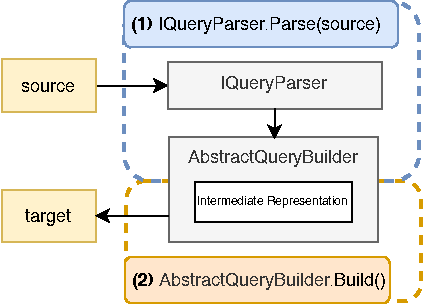
\includegraphics[scale=1]{thesis/img/thesis/05_translate_process_queries.drawio.pdf}
  \caption{Translation process of query with (1) parsing and (2) building phase.}
  \label{fig:translation_process_query}
\end{figure}

The parser must be provided an entire method or a repository class to obtain sufficient context. Queries may lack important context, such as the database table and column names, which are only accessible through entity mapping. While this is not necessary for \acrshort{sql} queries, it is especially important for \acrshort{linq} queries, which abstract away the underlying database structure. Therefore, it is assumed that query translation occurs after entity translation is completed and the mapping is stored in the intermediate representation. This representation can then be passed to the query parser to look up metadata.

\begin{example}
\small
This example demonstrates a simple repository class using \acrshort{efcore} with one method. 
It could serve as an input to the translation tool. A method argument is captured in the query and used as a parameter. 
\begin{lstlisting}[language=CSharp]
class CustomerRepository(DbContext context)
{
    List<Customer> GetCustomersWithLimitOver(int limit)
    {
        return ctx.Customers
            .Where(c => c.CreditLimit > limit)
            .OrderByDescending(c => c.Name)
            .ToList();
    }
}
\end{lstlisting}
\qed
\end{example}

\subsection{Query builder}

Query builder constructs the abstract instructions internally, without exposing them to the parser. The abstract query builder instead exposes a set of methods and builds these instructions internally.

As the parser begins processing a query or any subquery, it calls the method \texttt{Push}. When leaving the nesting, it calls its counterpart \texttt{Pop}. The builder keeps track of the start of the nesting and, when it ends, collects all the instructions, wrapping them in the \texttt{SUBQUERY} instruction. When parsing is complete, the list of instructions should contain a single element. It must be either a \texttt{SUBQUERY} or a \texttt{SET\_OPERATION} instruction.

Methods such as \texttt{From}, \texttt{Project}, \texttt{Select}, \texttt{Join}, \texttt{OrderBy}, \texttt{GroupBy}, and \texttt{Having} correspond directly to the respective instruction types, including their arguments. These are exposed as public methods, allowing the parser to construct the query incrementally while abstracting away the internal representation.

Listing~\ref{lst:aqb} presents the structure of the \texttt{AbstractQueryBuilder} class. All methods that build the internal instruction representation are public and fully implemented. Two abstract methods are declared and must be implemented by concrete framework implementations. The \texttt{BuildSQL} method serves to generate output queries using raw \acrshort{sql}. For Dapper and PetaPoco, which support only \acrshort{sql} queries, the purpose is straightforward. Other frameworks that primarily use \acrshort{linq} also offer an option to execute raw \acrshort{sql}. In such cases, this method enables that functionality if desired by the user. Otherwise, the \texttt{Build} method is exposed to generate a \acrshort{linq}-based variant. The builder does not declare any private abstract methods. As query structures differ significantly across frameworks, the internal implementation is left entirely to a developer.

w
 \begin{lstlisting}[caption={AbstractQueryBuilder class structure}, language=pseudo, label={lst:aqb}]
abstract class AbstractQueryBuilder
    
public: 
    Push() {...}
    Pop() {...}
    SetOperation(operationType) {...}
    From(table, alias) {...}
    Project(table, attribute, alias, aggregationFn) {...}
    Select(condition) {...}
    Join(table1, table2, joinType, condition) {...}
    OrderBy(table, attribute, direction) {...}
    GroupBy(table, attribute) {...}
    Having(condition) {...}
    
    abstract Build() : string;
    abstract BuildSQL() : string;
 \end{lstlisting}

 Before generating each (sub)query, the builder may need to reorder the corresponding instructions. For example, in \acrshort{sql}, projection appears at the beginning of the query but references attributes defined later. Whereas in \acrshort{linq} it typically comes at the end, just before result materialization.


 
%alg returns just the query - mention in the text how to wrap it
\begin{algorithm}[!htp]
    \small
    \DontPrintSemicolon

    \SetKw{return}{return}
    
    \KwIn{$inst$ -- abstract instructions built in parsing phase\;}
    \myinput{$sb$ -- string builder\;}
    
    BuildProjectionPart($sb$, $inst$)\;
    BuildFromPart($sb$, $inst$)\;
    BuildJoinPart($sb$, $inst$)\;
    BuildWherePart($sb$, $inst$)\;
    BuildGroupByPart($sb$, $inst$)\;
    BuildHavingPart($sb$, $inst$)\;
    BuildOrderByPart($sb$, $inst$)\;

    \return{$sb$.ToString()}
    \caption{Query builder}
    \label{alg:query_builder_main}
\end{algorithm}
 

\subsection{Query parser}

% stejné jako v předchozí kapitole, jen má parser přístup k IR

\subsection{Translation process}


\begin{figure}[!htp]
  \centering
  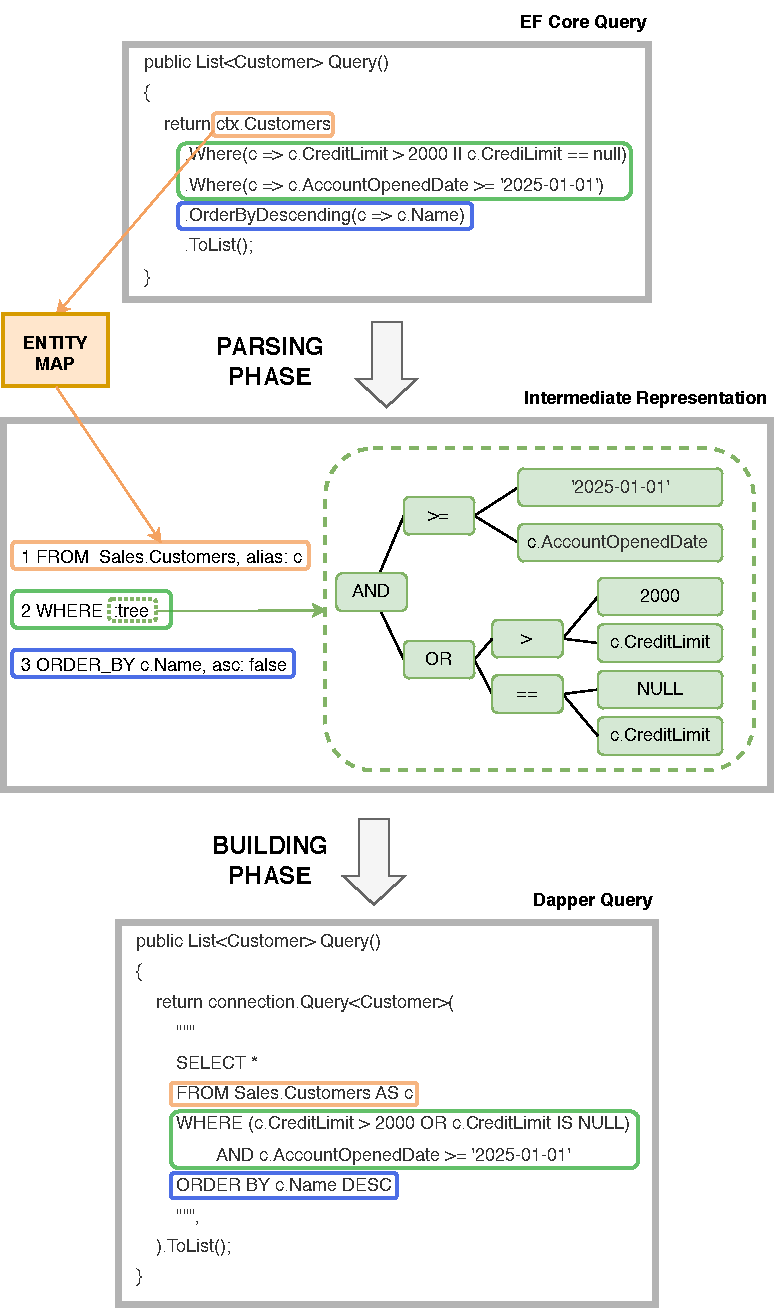
\includegraphics[scale=1]{thesis/img/thesis/05_parsing_building_queries.drawio.pdf}
  \caption{Translation of \acrshort{efcore} LINQ query to SQL in Dapper.}
  \label{fig:translation_complete}
\end{figure}